\documentclass[12pt, notitlepage]{article}
\usepackage{amsmath}
\usepackage{amssymb}
\usepackage{graphicx}
\usepackage{amsthm}
\usepackage{listings}
\usepackage{color}
\usepackage{float}

\definecolor{dkgreen}{rgb}{0,0.6,0}
\definecolor{gray}{rgb}{0.5,0.5,0.5}
\definecolor{mauve}{rgb}{0.58,0,0.82}

\lstset{
	frame=single,
	language=Java,
	belowskip=3mm,
	showstringspaces=false,
	columns=flexible,
	captionpos=b,
	basicstyle={\small\ttfamily},
	numbers=left,
	numbersep=5pt,
	%numbers=none,
	numberstyle=\tiny\color{gray},
	keywordstyle=\color{blue},
	commentstyle=\color{dkgreen},
	stringstyle=\color{mauve},
	breaklines=true,
	breakatwhitespace=true,
	tabsize=3
}


\providecommand{\abs}[1]{\lvert#1\rvert}
\providecommand{\norm}[1]{\lVert#1\rVert}

\newtheorem{thm}{Theorem}
\newtheorem{lemma}[thm]{Lemma}
\newtheorem{fact}[thm]{Fact}
\newtheorem{cor}[thm]{Corollary}
\newtheorem{eg}{Example}
\newtheorem{ex}{Exercise}
\newtheorem{defi}{Definition}
\newtheorem{hw}{Homework}
\newenvironment{sol}
  {\par\vspace{3mm}\noindent{\it Solution}.}{\qed}

\newcommand{\fib}{\mbox{fib}}
\newcommand{\ov}{\overline}
\newcommand{\cb}{{\cal B}}
\newcommand{\cc}{{\cal C}}
\newcommand{\cd}{{\cal D}}
\newcommand{\ce}{{\cal E}}
\newcommand{\cf}{{\cal F}}
\newcommand{\ch}{{\cal H}}
\newcommand{\cl}{{\cal L}}
\newcommand{\cm}{{\cal M}}
\newcommand{\cp}{{\cal P}}
\newcommand{\cz}{{\cal Z}}
\newcommand{\eps}{\varepsilon}
\newcommand{\ra}{\rightarrow}
\newcommand{\la}{\leftarrow}
\newcommand{\Ra}{\Rightarrow}
\newcommand{\dist}{\mbox{\rm dist}}
\newcommand{\bn}{{\mathbf N}}
\newcommand{\bz}{{\mathbf Z}}

\setlength{\parindent}{0pt}
%\setlength{\parskip}{2ex}
\newenvironment{proofof}[1]{\bigskip\noindent{\itshape #1. }}{\hfill$\Box$\medskip}

\usepackage{enumerate,fullpage, proof}
\newcommand{\Infer}[2]{\infer{#2}{#1}}

\title{Homework 3}
\author{Team: nogg\footnote{E-mail: \texttt{kimi.ysma@gmail.com}}\footnote{Team member: Ma Yesheng, Zhao Ming, Hu Hu, Zou Yikai, Fan Minghua}}

\begin{document}

{\bf\small CS214: Algorithms and Complexity}\hfill{\bf\small 2016 Fall}
{\let\newpage\relax\maketitle}


\textbf{Exercise 1}
\begin{enumerate}
\item
\begin{defi}[Cut Lemma]
\vspace{-0.85cm}
Suppose edge set $X$ is good, pick any vertex set $S\subseteq V$ s.t. there is no edge in $X$ that goes from $S$ to $V\backslash S$. Let $e\in E$ be the edge going from $S$ to  $V\backslash X$ with the cheapest weight, then $X\cup \{e\}$ is also good.
\end{defi}
\begin{proof}
	\mbox{ }
\begin{enumerate}[(1)]
	\item If the cheapest edge $e$ happens to be in the tree $T$, then the case is trivial.
	\item If the cheapest edge $e$ is not in the tree $T$, since $T$ is already a tree, adding any edge to it will result in a circle and there must exist another edge $e'$ which also goes from $S$ to  $V\backslash X$. If we remove this edge $e'$, we will get another graph $T' = T\cup \{e\} -\{e'\}$. Next, we are going to prove that it is also a minimum spanning tree.
	\begin{enumerate}[(a)]
		\item First, we prove that $T'$ is a tree. Since $T$ is a tree, adding a edge to it will form a circle. Then we remove the  edge $e'$ from $T\cup\{e\}$ where $e'$ is part of a circle and removing it will not disconnect the graph, hence $T' = T\cup\{e\} - e'$ is also connected. On the other hand, in the connected graph $T'$, $|E|-|V| = 1$, therefore $T'$ is a tree.
		\item Next, we prove that $T'$ is a minimum spanning tree. Since substitute $e'$ for $e$ will not affect spanning property of minimum spanning tree, all we need to prove is it takes minimum weight. From the equation $weight(T') = weight(T)-w(e)+w(e')$, since $e'$ is chosen to be the edge with minimum weight, thus $weight(T') < weight(T)$. Therefore $T'$ is a minimum spanning tree.
		
	\end{enumerate}
\end{enumerate}
Combine (1) and (2), cut lemma is proved.\\\\
\end{proof}

\item 
\begin{proof}
	\mbox{ }
	
	\qquad To prove this lemma, we construct a situation that meets the conditions of this lemma. And then we will prove that it must exist. In the following, we will illustrate that how we construct it and prove it must exit.
	
	\textbf{The construct process}
	\begin{enumerate}[(1)]
		\item Construct the initial cut $S$\\
		We divided X to different connected sets $X_1,X_2,...X_n$. Then consider the following situations, we will construct a connected initial cut $S$ which includes only one vertex of the given edge $e$ and no edge from $X$ crosses it.
		\begin{enumerate}[a.]
			\item If only one vertex of the given edge $e$ is in a $X_i$, then we construct the initial cut $S$ with vertice in $X_i$.
			\item If two vertice of $e$ are in $X_i$ and $X_j$, then we can construct initial $S$ with vertice in $X_i$ or $X_j$.
			\item If none of vertice of $e$ it in any $X_i$. Then choose any $X_i$, there must be a route $g$ in MST connects $e$ and $X_i$. Here we construct initial $S$ with vertice in route $g$(include one vertex of $e$) and $X_i$. If $g$ goes through any other $X_j$, add it to $S$.
		\end{enumerate}
		\item Update the cut $S$\\
		We update the initial $S$ constructed in (1), then we will ensure that $e$ is the minimum weight edge of $G$ crossing this cut.
		\begin{enumerate}[a.]
			\item Find the minimum weight edge $f$ crossing $S$ to $V\backslash X$. 
			\item If $f$ is not $e$, add the other vertex of $f$ to $S$.If the other vertex of $f$ is included in other $X_j$, add the whole vertice in $X_j$ to $S$. Return to step a.\\
			According to \textbf{Cut Lemma}, $f$ must belongs to $E(T)$. And the $S$ must be connected all the time we add vertex to it. \\
			Here are 2 situations we should consider. 
			\begin{enumerate}[I.]
				\item The other vertex of $f$ is the other vertex of $e$. As the picture shown blow. Here $f$ and $e$ are all belong to $E(T)$, and vertice in $S$ are connected by edge in $E(T)$, so it must be a cycle in $E(T)$, which is impossible.
				\begin{figure}[H]
					\center
					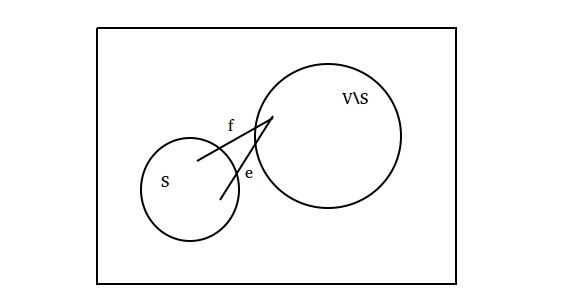
\includegraphics[width=0.6\linewidth]{p1.jpg}\vspace{-5pt}\nonumber
				\end{figure}
				\item The other vertex of $e$ is in the $X_j$ that include the other vertex of $f$. As the picture shown below. Here $f$ adn $e$ are all belong to $E(T)$, and vertice in $S$ and $X_j$ are connected by edge in $E(T)$, so it must be a cycle in $E(T)$, which is impossible.
				\begin{figure}[H]
					\center
					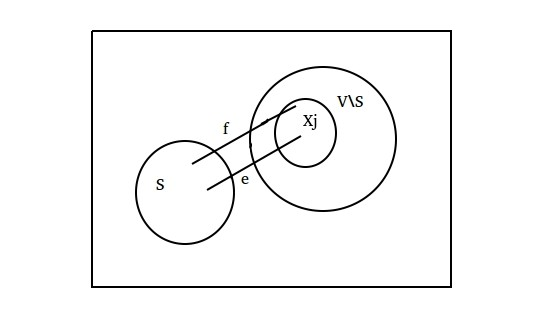
\includegraphics[width=0.6\linewidth]{p2.jpg}\vspace{-5pt}\nonumber
				\end{figure}
			\end{enumerate}
			\item If $f$ is $e$, stop.
			Here, for cut $S$, there is no edge from $X$ crosses it. And $e$ is a minimum weight edge of $G$ crossing this cut.
		\end{enumerate}
	\end{enumerate}
	To sum up, we can always construct a cut $S$ that meets the conditions in reverse cut lemma. Therefore, this lemma is proved.\\
\end{proof}

\item 
\end{enumerate}


\textbf{Exercise 2}
\begin{enumerate}
\item
\item
\textbf{If:}\\
Proof by contradiction. Assuming that u and v are connected in $G_c$, but not connected in $T_c$, which means two things:\\
1. In T, there exists at least one edge with weight more than c in the route from u to v. \\
2. In $G_c$, there is more than one routes from u to v with all edges' weight less than or equal to c.\\
It's obvious that the special edge in 1 is not within $G_c$.Then according to the construction process of MST T using Kruskal algorithm,  if there is no cycle, then we first add the lowest-weight edge into the MST. So since the special edge is of more weight than all the edges in the routes of Gc which connect u and v, then it shouldn't be added into T until one route from u to v is constructed. Then we can know that in MST T, u and v are connected.\\
\textbf{Only if:}\\
Since $T_c$ is a subset of $G_c$, then if u,v are connected in $T_c$, then it is connected in $G_c$.
\end{enumerate}

\end{document}
